\begin{figure}[t!]
\begin{small}
    \begin{center}
    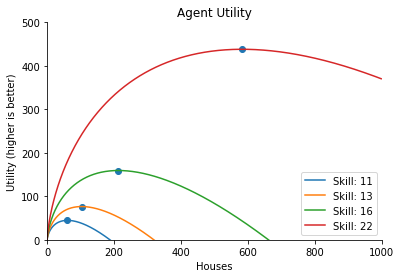
\includegraphics[width=0.617\linewidth]{figures/agent_utility.png}
    \end{center}
    \caption{Agent utility, as defined in Equation \ref{eq:agent_utility}, in a simplified setting where utility only depends on the number of houses built, for four agents with different skills $\skill_0 < \ldots < \skill_3$. For clarity of this visualization, each agent is assumed to receive a fixed income per house, which increases with skill, as described in Section \ref{sec:env_rules_and_dynamics}. For each house built, each agent is also assumed to have exerted a fixed amount of labor. Hence, in this simple example, agent utility only depends on the number of houses built. Each agent experiences a law of diminishing returns (marginal utility decreases as income grows). As agent skill increases, the point of maximal utility is reached at a higher number of houses built.}
    \label{fig:agent_utility}
\end{small}
\end{figure}


\subsection{Using Machine Learning to Optimize Agent Behavior}
\label{sec:agent_utility}

To ground our simulation in economic theory, we model the reward that the agents learn to optimize as a {\em utility function}.
Recall that $\endow_{i,t}$ denotes the endowment of resources (stone and wood) and coin owned by an agent at time $t$.  At time $t$, the utility experienced by an agent $i$ is a function of the number of coins that it has accumulated $\money_{i,t}$, and the total labor that it has exerted $\labor_{i,t}$.
In particular, we adopt a  utility function that is concave and increasing in money, and linearly decreasing in labor:
\eq{\label{eq:agent_utility}
    \util_{i}(\endow_{i,t}, \labor_{i,t}) = \crra\brck{\mon{i}{t}} - \labor_{i, t},
    \quad
    \crra\brck{\income} = \fr{\income^{1-\isoeta}-1}{1-\isoeta}, \quad
    \isoeta > 0.
}


Here,
$\labor_{i, t}$ is the cumulative labor associated with the actions taken by the agent up to time $t$,
and the concave isoelastic utility $\crra$ models diminishing marginal utility over money \citep{debreu_representation_1968}. Parameter $\isoeta$ controls the degree of nonlinearity: higher  $\isoeta$ represents larger deviations from linear behavior.
We assume that all agents share the same form of utility function. This utility function is visualized in Figure \ref{fig:agent_utility} for a simple setting without trading and where there is no labor cost associated with moving or gathering resources.

Rational economic agents optimize their total discounted utility over time, with
\eq{\label{eq:agentproblem}
    \forall i:
    \max_{\policy_i}
    \E_{
    \ac_i    \sim \policy_i,
    \Ac_{-i} \sim \bm{\policy}_{-i},
    \st'     \sim \trans
    }\brcksq{
        \sum_{t = 1}^\eplen \df^t
        \underbrace{\brck{
            \util_i( \endow_{i,t}, \labor_{i,t} )
            - \util_i( \endow_{i,t-1}, \labor_{i,t-1} )
        }}_{=\hspace{2pt} \rew_{i,t}}
        + \util_i( \endow_{i,0}, \labor_{i,0} )
    }.
}

In the paradigm of RL, this is achieved  by defining the instantaneous reward $\rew_{i,t}$ for agent $i$ as the change in utility of  agent $i$   at time $t$.


Equation \ref{eq:agentproblem} describes a multi-agent optimization problem, when the agents are simultaneously optimizing their behavior, since the utility for agent $i$ depends on the behaviors of other agents (for example, their gathering, building and trading actions).
For instance, another agent might block an agent's access to resources, which would impact how many houses the agent can build in the future and hence its future utility.

In general, such optimization problems are described as partially-observable multi-agent Markov games, and optimal solutions correspond to refinements of Nash equilibria.  A set of policies form a Nash equilibrium as long as no agent wants to unilaterally deviate from its own policy. Refinements such as  subgame-perfect equilibria also require rational, off-equilibrium behavior. Although computing equilibria for complex environments such as this remains out-of-reach,  we will see that RL can nevertheless be used to achieve sensible, emergent behaviors (and behaviors that also drive good tax policy, when coupled with the use of the AI Economist).


\paragraph{Deep RL agents.}
We make use of a deep neural network to model agent policies,
\eq{
 \ac_{i, t} \sim \policy(\ob^\text{world}_{i, t}, \ob^\text{agent}_{i, t}, \ob^\text{market}_{i, t}, \ob^\text{tax}_{i, t}, \hidden_{i, t-1}; \mweight).
}

The output of this policy network includes a probability distribution over actions, with $\ac_{i, t}$ sampled from this distribution. Not represented in the notation, the policy network also generates an updated hidden state $\hidden_{i, t}$.
The inputs to the network include the agent-specific hidden state and agent-specific observations, which are decomposed as follows:
\begin{itemize}
    \item $\ob^\text{world}_{i, t}$: spatial observations from the nearby world.
    \item $\ob^\text{agent}_{i, t}$: the \textit{public} agent state (such as resource and coin endowments), as well as the \textit{private} agent state (such as skill values and labor performed).
    \item $\ob^\text{market}_{i, t}$: the full market state, including available offers to buy/sell resources.
    \item $\ob^\text{tax}_{i, t}$: the tax rates in effect.\footnote{We include tax information even for the free-market, when all tax rates are zero. This ensures that the structure of the observations is the same for all taxation schemes.}
\end{itemize}

\begin{figure}[t!]
    \begin{small}
        \begin{center}
            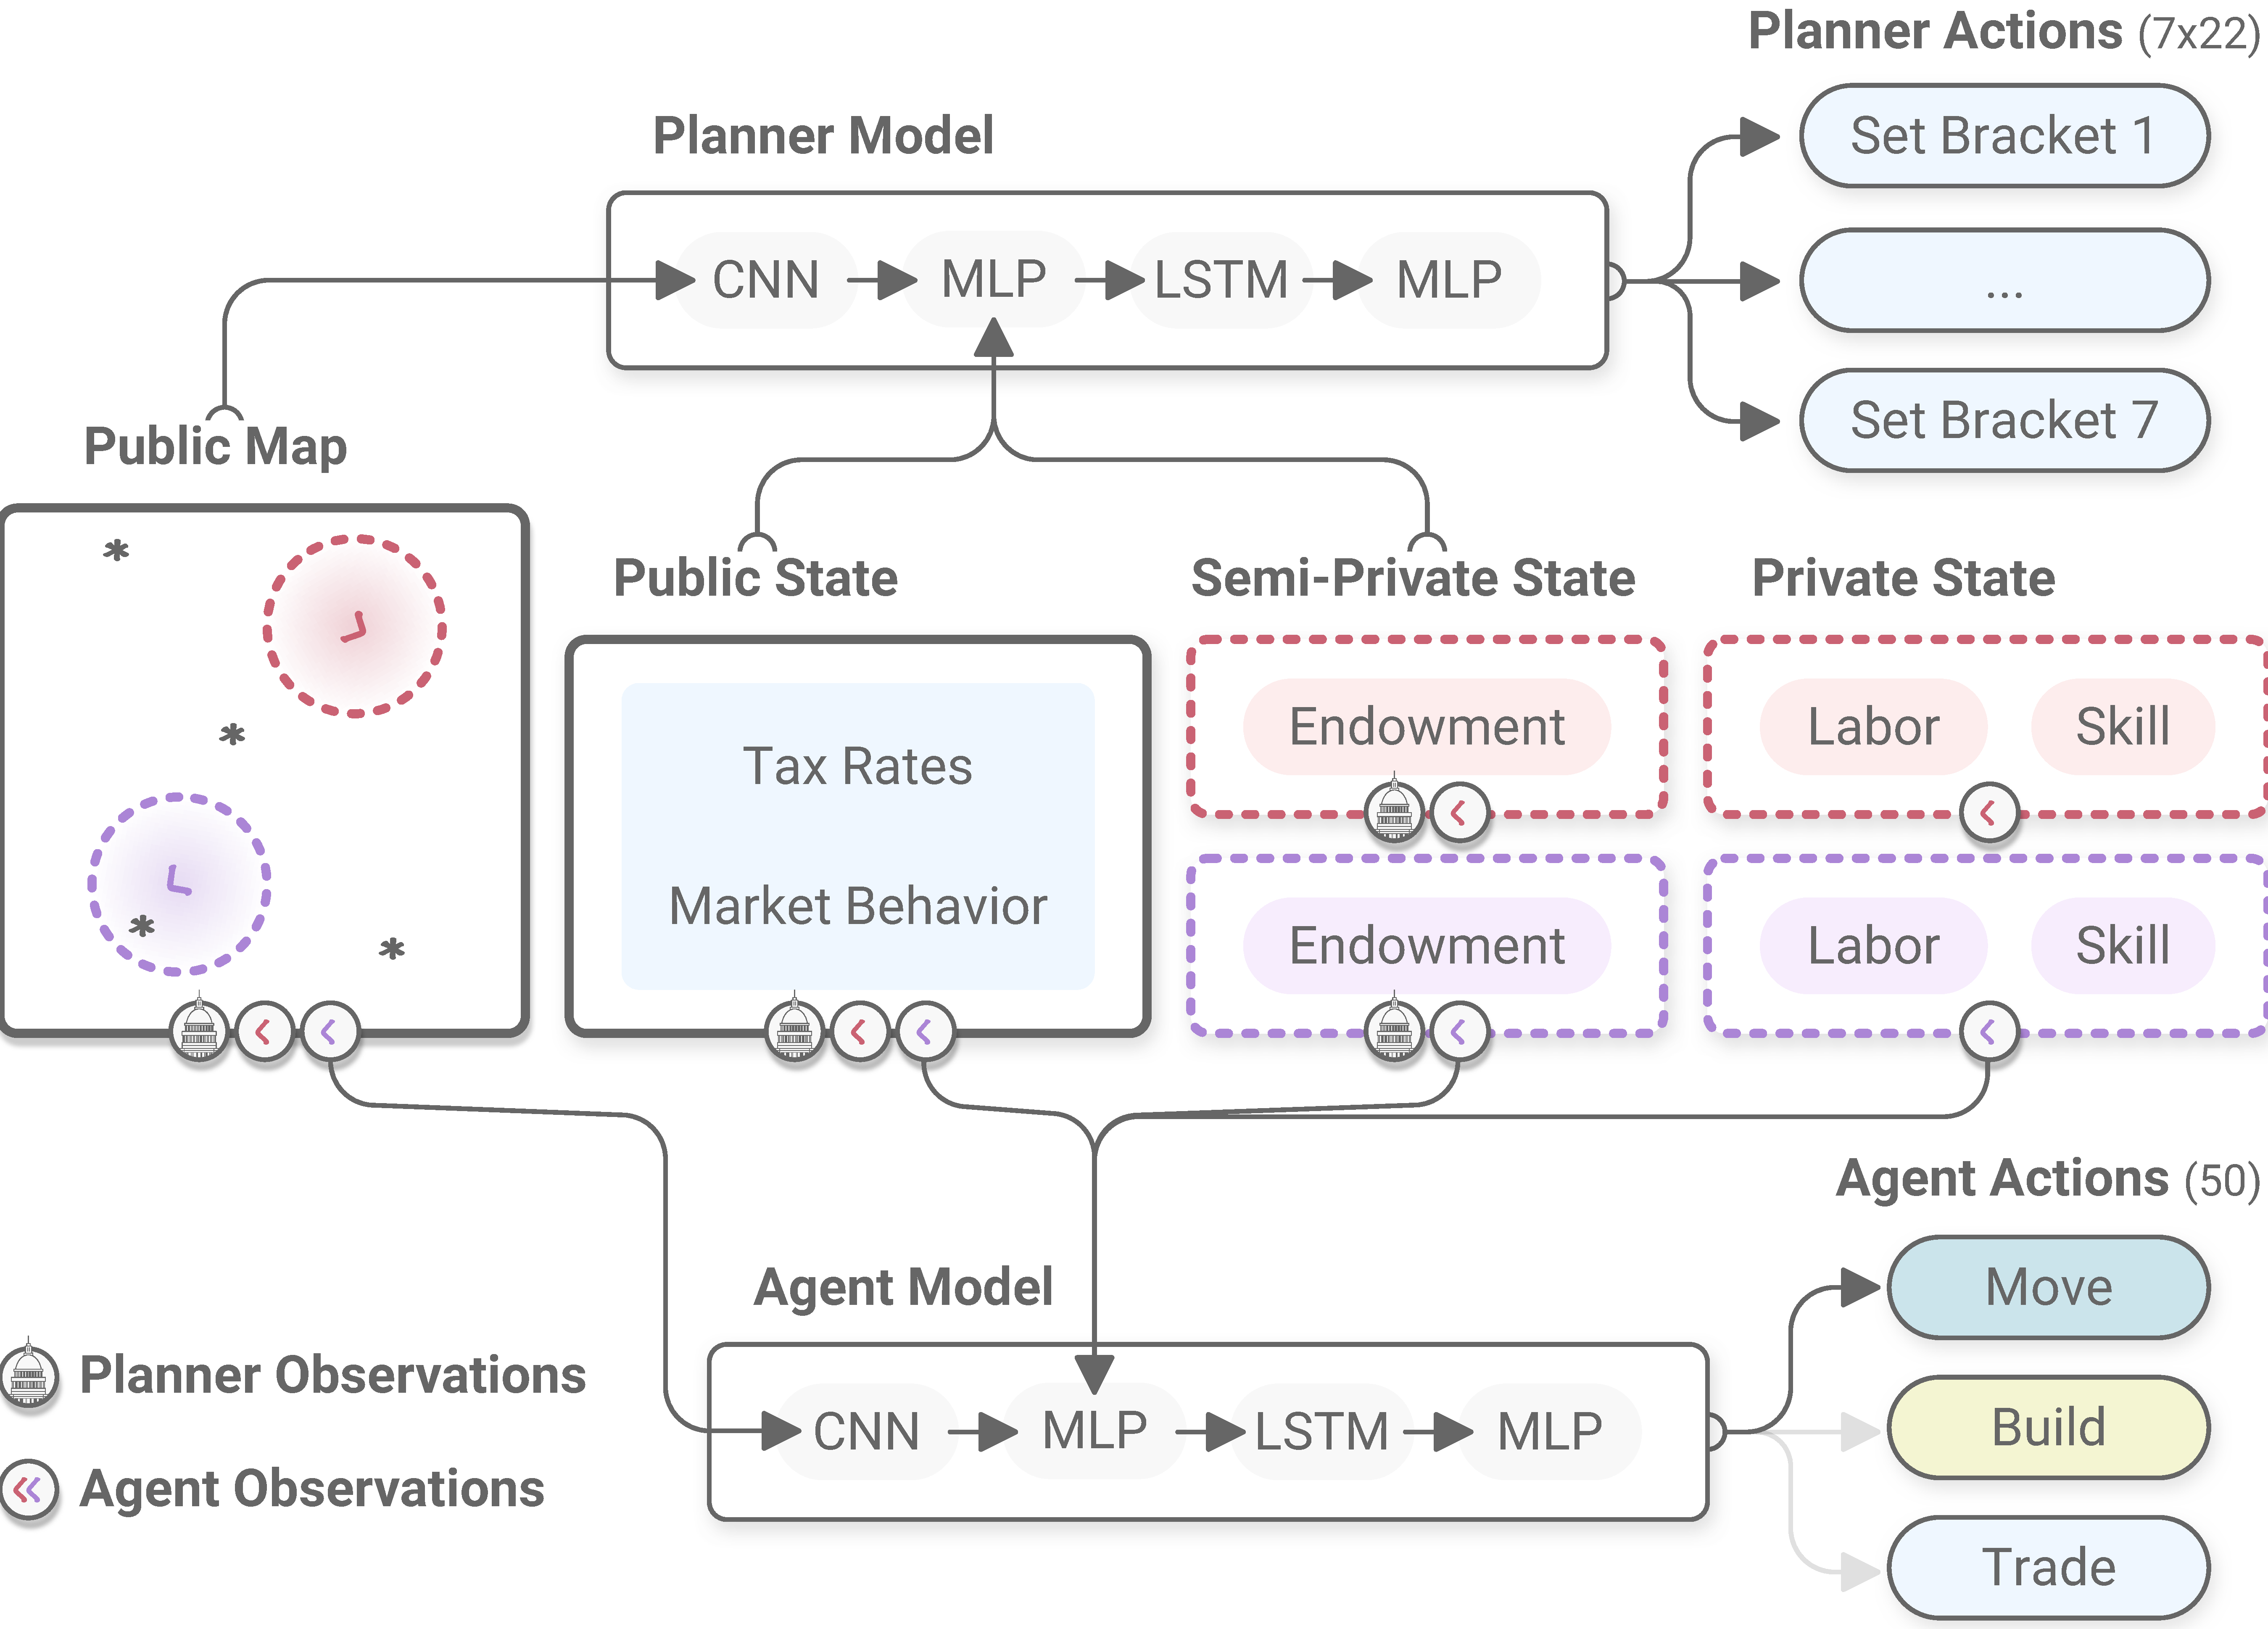
\includegraphics[width=0.8\textwidth]{figures/postprocessed/econ-rnn3.pdf}
        \end{center}
        \caption{
        Schematic overview of the general network architecture used in our work.
        Spatial observations are processed by a stack of two convolutional layers (CNN) and flattened into a fixed-length feature vector.
        This feature vector is concatenated with the remaining observation inputs and the result is processed by a stack of two fully connected layers (MLP).
        The output is then used to update the hidden state of an LSTM and action logits are computed via a linear projection of the updated hidden state.
        Finally, the network computes a softmax probability layer for each action head.
        For the agent policy, there is a single action space and action head.
        For the tax policy, there is a separate action space and action head for each tax rate the tax policy controls (described below).
        }
        \label{fig:neural_network_policies}
    \end{small}
\end{figure}

Section \ref{sec:details_of_environment} of the appendix provides exact details of the information available in the agents' observations.
The learned hidden state $\hidden_{i,t}$ is used to encode the history of past observations.
Figure \ref{fig:neural_network_policies} depicts the general network architecture used here.


\paragraph{Emergent Behavior of AI Agents.}
Figure \ref{fig:rollout} provides a breakdown of an example rollout of play by AI agents across a single episode, once training has proceeded for a large number of episodes.
Each agent has a unique color. Agents are ordered from low to high skill as dark-blue, light-blue, yellow, and orange, corresponding to payoffs of 11.3, 13.3, 16.5, and 22.2 coins per house, respectively.

This rollout reveals an interesting specialization of effort.
The dark- and light-blue agents focus entirely on collecting wood and stone (respectively), the orange agent focuses almost entirely on building houses, and the yellow agent builds several houses early on before switching to collecting and selling.

This pattern of behavior and division of labor is typical of agents trained in this simulated environment, and stems from the different incomes each agent can earn per house it builds, as well as the agents' initial locations in the world.
In particular, the low skilled dark- and light-blue agents learn to shift their strategies entirely away from building houses.
These agents earn their income by selling resources to the higher skilled agents, who choose to earn income through building (Figure \ref{fig:rollout}, middle).
The yellow agent earns enough income from building to do so early on, making use of the nearby resources, but then switches strategies.

This specialization is a consequence of agents learning to maximize their own individual objectives.
We do not impose these roles or behaviors directly. Rather, this  specialization arises as a result of differently skilled workers learning to balance their income and effort.
This emergent behavior helps to validate the framework as an economic simulation, by reproducing a standard feature of real world economies, that of specialization.
Standard economic intuition states that agents should specialize in whichever means of production allows them to most efficiently convert their labor to income, and this is consistent with the behaviors that the AI agents discover.


Even with specialization, the agents' incomes can vary considerably.
While a free-market economy maximizes productivity, it provides no guarantee on income equality.
This is evident in the highly unequal incomes  experienced by the AI agents.




\begin{figure}[t!]
    \begin{center}
        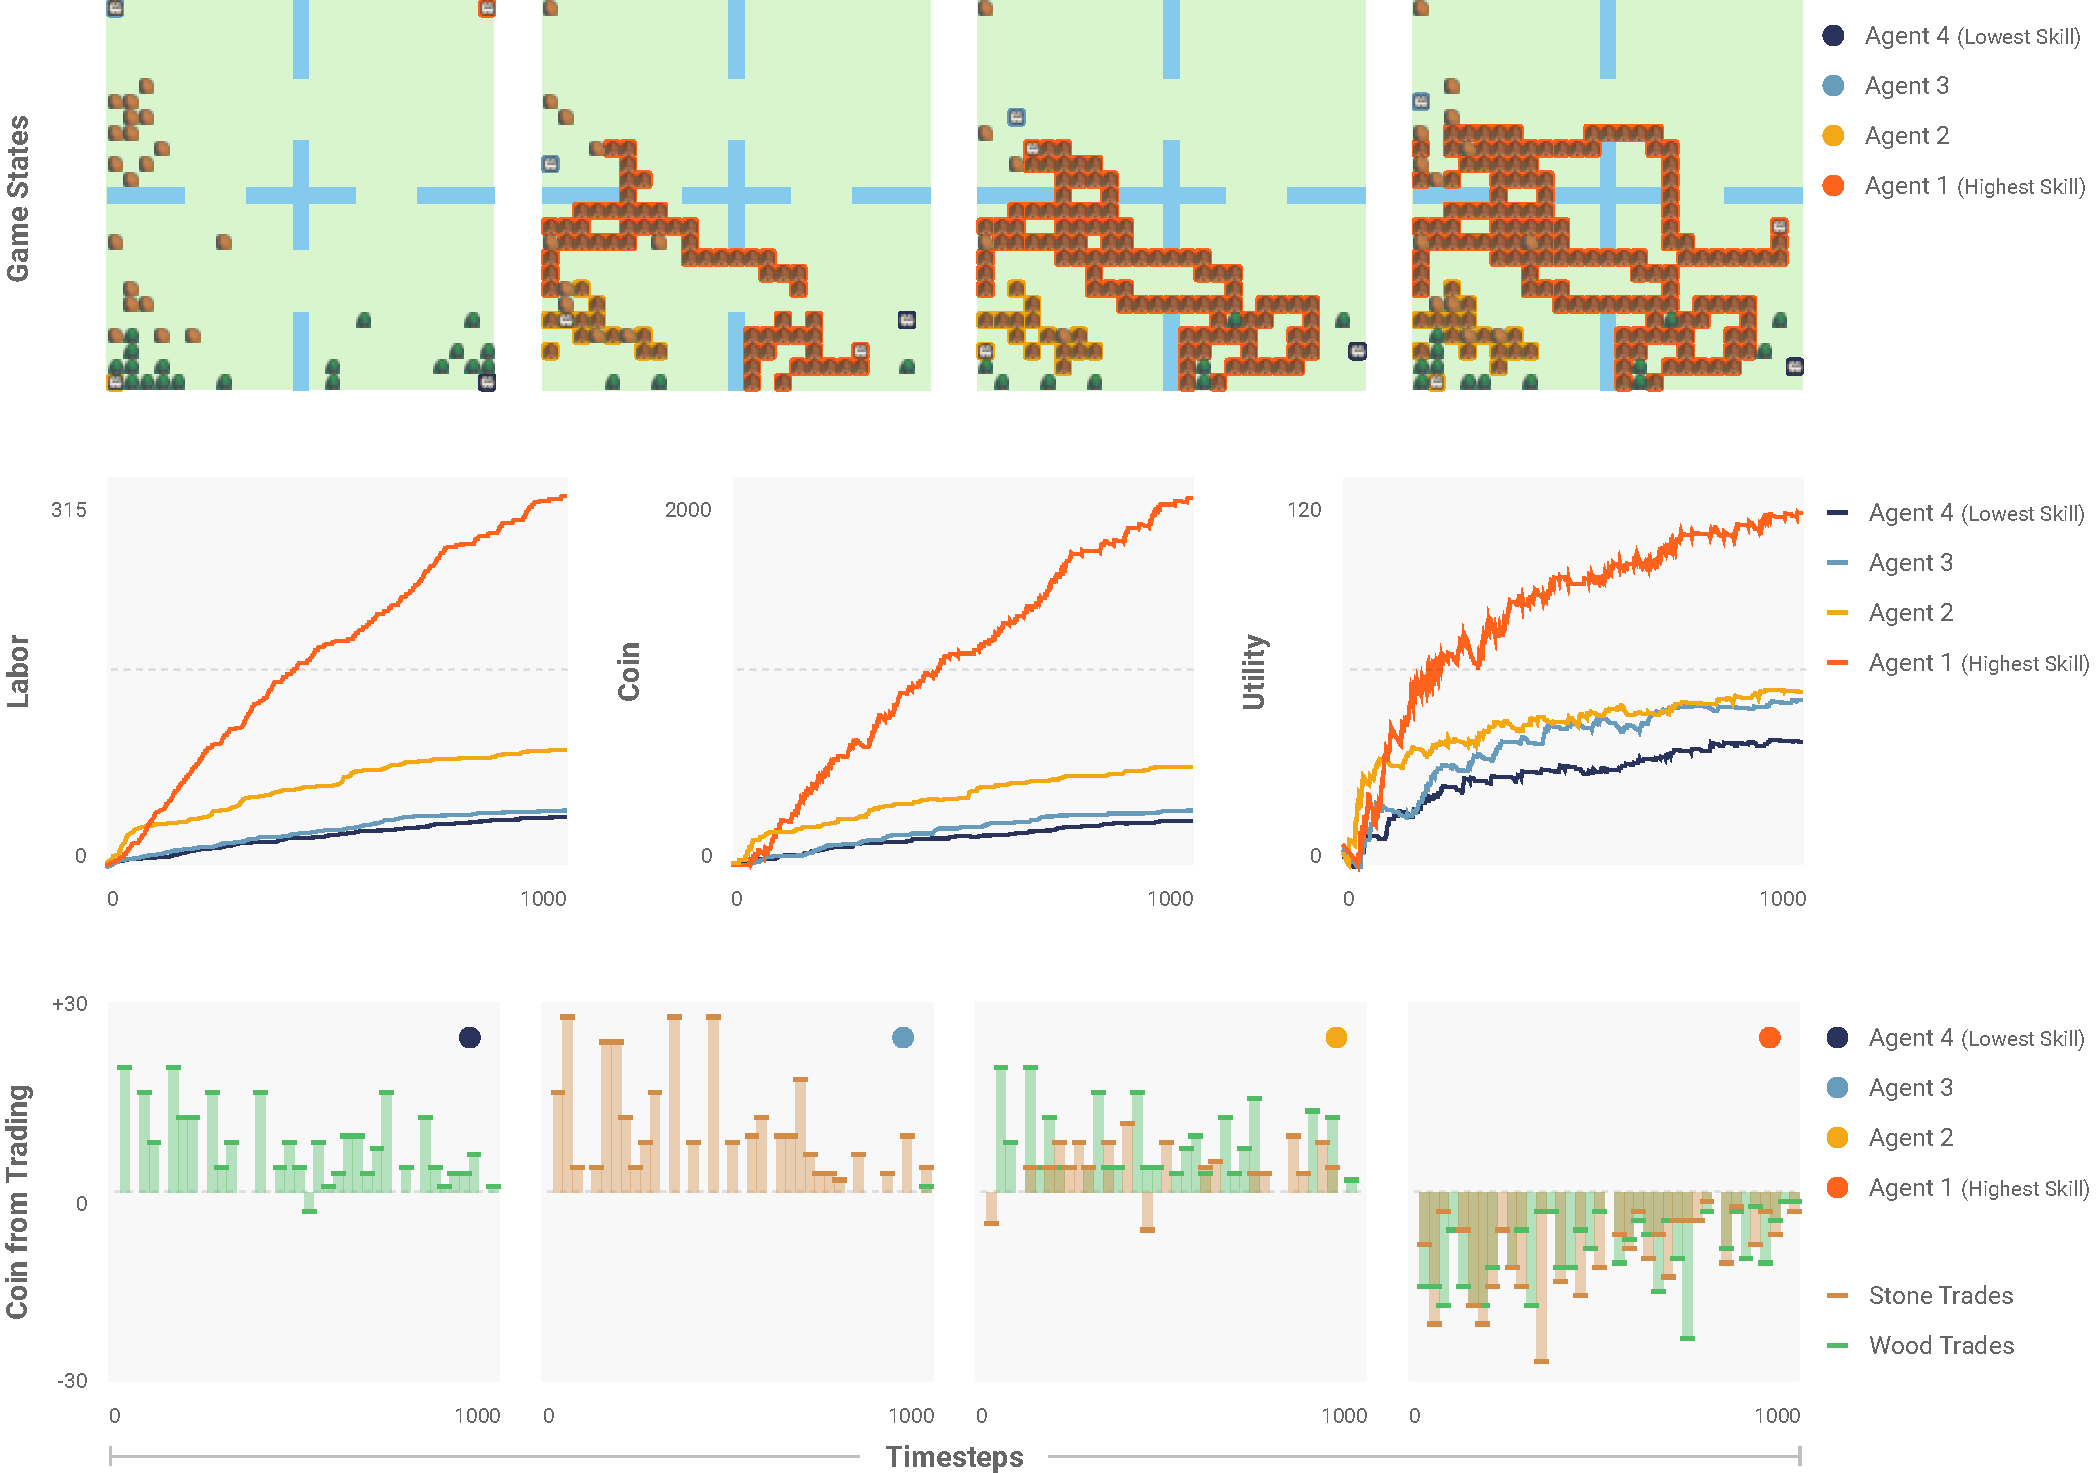
\includegraphics[width=0.95\textwidth]{figures/postprocessed/breakdown-post-group.pdf}
  \end{center}
  \caption{
  Breakdown of an example rollout in a no-tax environment.
  Agents labels are sorted according to each agent's building skill (dark-blue is lowest, orange is highest). These correspond to agent payoffs of 11.3, 13.3, 16.5, and 22.2 coins per house.
  The top panels illustrate the world state, including agent locations, available resources, and built houses, as the episode progresses.
  The middle panels illustrate the accumulated labor, coin, and utility of each agent over the episode.
  Highly skilled agents ultimately experience more utility.
  The bottom panels illustrate the net coin received/spent from trading over the episode, for each of the four agents.
  Each bar represents the net coin within a window of 25 timesteps, with upward bars indicating net income (agent predominantly sold), downward bars indicating net cost (agent predominantly bought), and color indicating the resource type.
  Agents with lower building skill choose to earn income through gathering resources and selling them to the highly skilled agents.
  }
  \label{fig:rollout}
\end{figure}